% =====================================================================
% StaticKD -- supplementary material for the IEEE Access manuscript (main.tex)
% Floats moved out of the main text on 2026-11-01; content unchanged.
% Compile: pdflatex supplementary && bibtex supplementary && pdflatex supplementary && pdflatex supplementary
% =====================================================================
\documentclass[journal,onecolumn]{IEEEtran}
\usepackage[T1]{fontenc}
\usepackage[utf8]{inputenc}
\usepackage[nocompress]{cite}
\usepackage{amsmath,amssymb}
\usepackage{graphicx}
\usepackage{booktabs}
\usepackage{array}
\usepackage[hyphens]{url}
\usepackage{algorithm}
\usepackage{algpseudocode}
\renewcommand{\thetable}{S\arabic{table}}
\renewcommand{\thefigure}{S\arabic{figure}}
\renewcommand{\thealgorithm}{S\arabic{algorithm}}
\begin{document}
\title{Supplementary Material for ``StaticKD: Distilling a Multilingual IPTC News Topic Classifier into a Static Token-Logit Table for Lightweight CPU Inference''}
\author{Obi~Kastanya and Ananta~Dwi~Prayoga~Alwy}
\maketitle

This document contains the algorithm, tables, and figures that the main text refers to as Algorithm~S1, Table~S1--S4, and Fig.~S1--S7.

\begin{algorithm}[!htbp]
\caption{StaticKD Inference for One Article}
\label{alg:infer}
\begin{algorithmic}[1]
\Require article text $d$; tokenizer; table $\bar{T}\in\mathbb{R}^{|V|\times 17}$; bias $\bar{\mathbf{b}}\in\mathbb{R}^{17}$
\State $(t_1,\dots,t_n)\gets$ first 1,024 tokens of tokenize$(d)$, without unknown tokens
\State $\mathbf{z}\gets\frac{1}{n}\sum_{i=1}^{n}\bar{T}_{t_i}+\bar{\mathbf{b}}$ \Comment{look up and average table rows}
\State \Return $\arg\max_{y}\,z_y$ \Comment{one of the 17 IPTC topics}
\end{algorithmic}
\end{algorithm}

\begin{table}[!htbp]
\caption{Hyperparameters of All Models}
\label{tab:hparams}
\centering
\footnotesize
\setlength{\tabcolsep}{3pt}
\resizebox{0.7\textwidth}{!}{%
\begin{tabular}{@{}ll@{}}
\toprule
Component & Value \\
\midrule
\multicolumn{2}{@{}l}{\textit{StaticKD}} \\
\quad initial embedding & potion-multilingual-128M (500,353 $\times$ 256) \\
\quad max. tokens / vector dropout & 1,024 / 0.1 \\
\quad loss, $\tau$ & KL, $\tau=1$ \\
\quad token dropout & 0.2 \\
\quad optimizer embedding / head & SparseAdam $10^{-3}$ / AdamW $3\cdot 10^{-3}$, wd $10^{-4}$ \\
\quad batch, epoch, validation & 64, 6, 3\% of data (selects the epoch) \\
\quad ensemble & mean of 3 seed tables \\
\multicolumn{2}{@{}l}{\textit{fastText}} \\
\quad word tokens (fixed) & dim 100, lr 0.5, 15 epoch \\
\quad subword tokens (fixed) & dim 100, lr 0.5, 15 epoch \\
\quad GPT-4o labels & dim 100, lr 0.5, 25 epoch \\
\quad word n-grams, loss & 2, softmax, 2M buckets \\
\quad tokens & words (+ character 2--5-grams) or XLM-R subwords \\
\quad quantization & \texttt{quantize}, cutoff 300k, retrain \\
\multicolumn{2}{@{}l}{\textit{TF-IDF + SVM}} \\
\quad features & XLM-R subword uni+bigrams, min.\ df 3, max.\ 1,000,000, sublinear tf \\
\quad classifier (fixed) & LinearSVC, $C=0.50$ \\
\multicolumn{2}{@{}l}{\textit{MiniLM-L6 / DistilmBERT + KD}} \\
\quad optimizer & AdamW $5\cdot 10^{-5}$, wd 0.01, warmup 6\%, linear, fp16 \\
\quad batch, epoch, max. tokens & 32, 2, 256 \\
\quad $\tau$ & $\{1, 2\}$, chosen on dev \\
\bottomrule
\end{tabular}}
\end{table}

\begin{table}[!htbp]
\caption{Test Macro-F1 by Source of the Unified Test Set. MN-DS Is the Only Source Annotated Directly With IPTC Topics. MasakhaNEWS Is Human-Annotated Under Its Own Scheme. Last Column: StaticKD as a Percentage of the Teacher}
\label{tab:sources}
\centering
\footnotesize
\setlength{\tabcolsep}{3.5pt}
\resizebox{\textwidth}{!}{\begin{tabular}{@{}llrrccccccc@{}}
\toprule
Source & Label origin & $n$ & Lang. & Teacher & DistilmBERT & MiniLM & \textbf{StaticKD} & fastText (q) & TF-IDF+SVM & \% teacher \\
\midrule
CC-NEWS 2024--2026 & JSON-LD section & 6,050 & 29 & 0.651 & 0.629 & 0.634 & 0.624 & 0.579 & 0.609 & 96\% \\
MasakhaNEWS~\cite{adelani2023masakhanews} & human annotation & 3,339 & 16 & 0.695 & 0.545 & 0.582 & 0.556 & 0.341 & 0.434 & 80\% \\
L3Cube-IndicNews~\cite{mirashi2023indicnews} & publisher category & 2,361 & 10 & 0.709 & 0.501 & 0.680 & 0.639 & 0.328 & 0.342 & 90\% \\
MN-DS~\cite{petukhova2023mnds} & human annotation & 755 & 1 & 0.549 & 0.546 & 0.535 & 0.535 & 0.493 & 0.461 & 97\% \\
Bangla news~\cite{hossain2025banglanews} & publisher category & 139 & 1 & 0.835 & 0.730 & 0.817 & 0.748 & 0.150 & 0.010 & 90\% \\
IndoNews & publisher category & 100 & 1 & 0.885 & 0.846 & 0.856 & 0.862 & 0.852 & 0.873 & 97\% \\
\bottomrule
\end{tabular}}
\end{table}

\begin{table}[!htbp]
\caption{Factors Behind Per-Language Performance}
\label{tab:factors}
\centering
\footnotesize
\setlength{\tabcolsep}{3pt}
\resizebox{0.7\textwidth}{!}{%
\begin{tabular}{@{}lcc@{}}
\toprule
Test & Statistic & $p$ \\
\midrule
Spearman: agreement vs log(distillation data) & $\rho=0.31$ & 0.022 \\
Spearman: agreement vs number of training sites & $\rho=0.29$ & 0.033 \\
Spearman: agreement vs teacher confidence & $\rho=0.71$ & $<$0.001 \\
Kruskal--Wallis: across scripts & $H=10.37$ & 0.065 \\
Spearman (test): accuracy gap vs log(data) & $\rho=0.52$ & $<$0.001 \\
Spearman (test): StaticKD accuracy vs token coverage & $\rho=0.50$ & $<$0.001 \\
Spearman (test): accuracy gap vs token coverage & $\rho=0.49$ & $<$0.001 \\
\bottomrule
\end{tabular}}
\end{table}

\begin{table}[!htbp]
\caption{Licenses of the Assets Used and Released}
\label{tab:license}
\centering
\footnotesize
\setlength{\tabcolsep}{3pt}
\resizebox{0.7\textwidth}{!}{%
\begin{tabular}{@{}ll@{}}
\toprule
Asset & License \\
\midrule
Teacher \texttt{classla/multilingual-IPTC-news-topic-classifier} & CC BY-SA 4.0 \\
Embeddings \texttt{minishlab/potion-multilingual-128M} & MIT \\
MasakhaNEWS & CC BY-NC 4.0 \\
MN-DS, L3Cube-IndicNews, IndoNews & CC BY 4.0 \\
Bangla news~\cite{hossain2025banglanews} & not stated on the dataset card \\
EMMediaTopic 1.0 & CC BY-SA 4.0 \\
CC-News 2019--2021, CC-NEWS 2024--2026 & Common Crawl terms of use \\
\midrule
StaticKD code (release) & MIT \\
StaticKD models (release) & CC BY-SA 4.0 (inherited from the teacher) \\
Test-set manifest (release) & CC BY-SA 4.0 \\
\bottomrule
\end{tabular}}
\end{table}

\begin{figure}[!htbp]
\centering
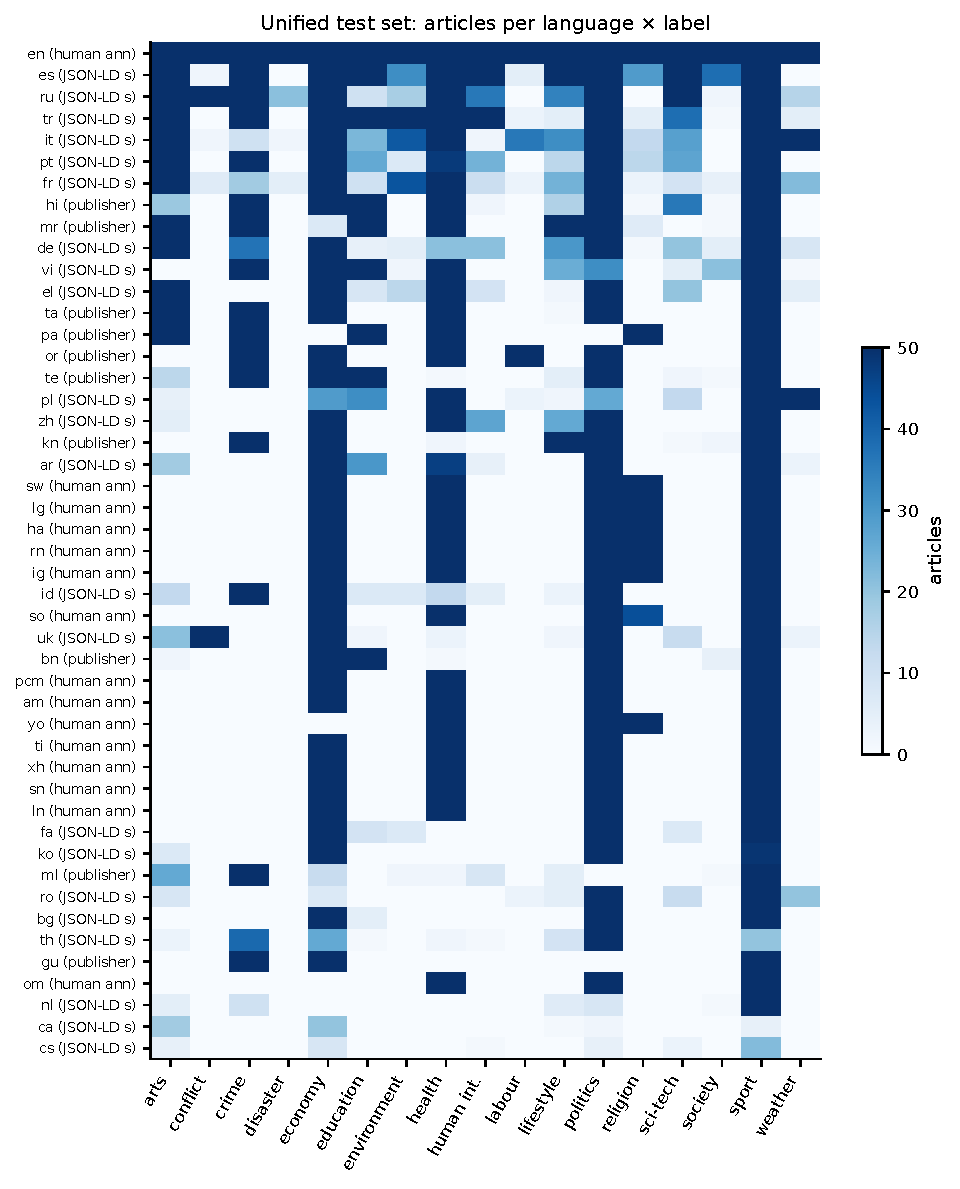
\includegraphics[width=\columnwidth]{figures/fig_testset_heatmap.pdf}
\caption{Articles in the unified test set per language and label (at most 50 per language--label pair). The label origin in brackets is the dominant one for that language.}
\label{fig:testset}
\end{figure}

\begin{figure}[!htbp]
\centering
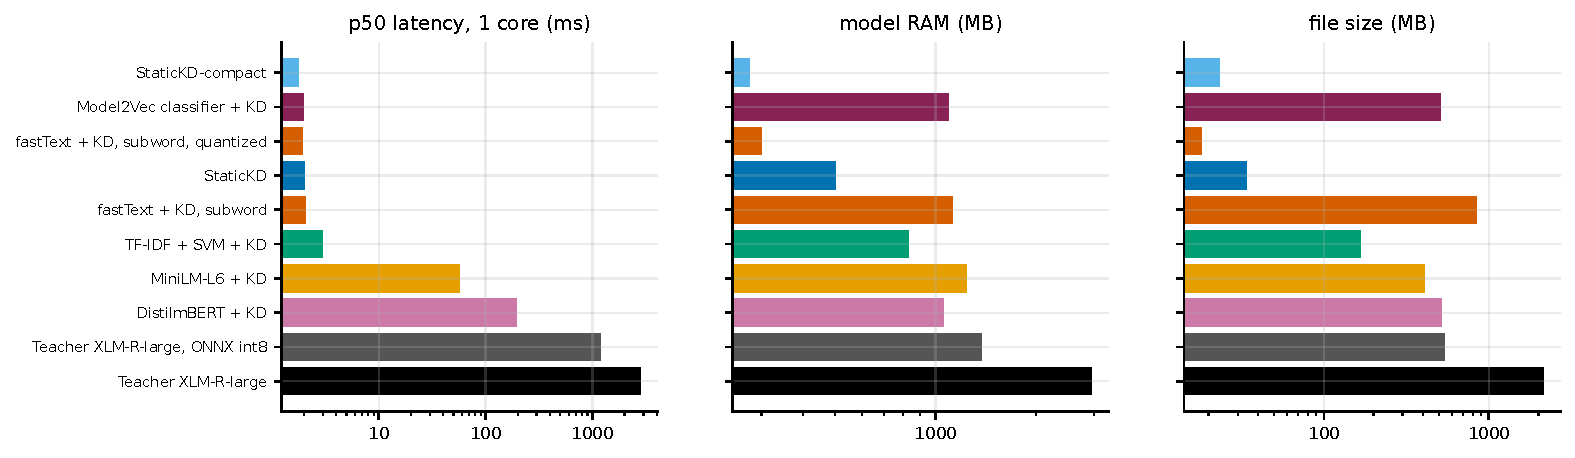
\includegraphics[width=0.9\textwidth]{figures/fig_latency_ram_size.pdf}
\caption{Latency per article, model RAM, and file size (log scale).}
\label{fig:latency}
\end{figure}

\begin{figure}[!htbp]
\centering
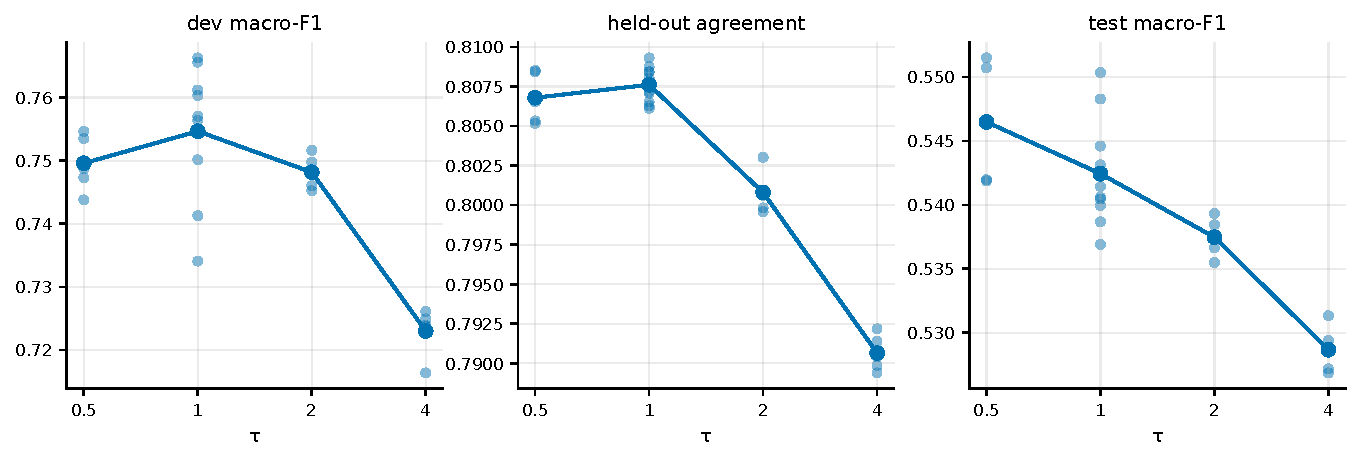
\includegraphics[width=0.9\textwidth]{figures/fig_temperature.pdf}
\caption{Effect of the distillation temperature. Each dot is one seed. The line connects the means.}
\label{fig:temperature}
\end{figure}

\begin{figure}[!htbp]
\centering
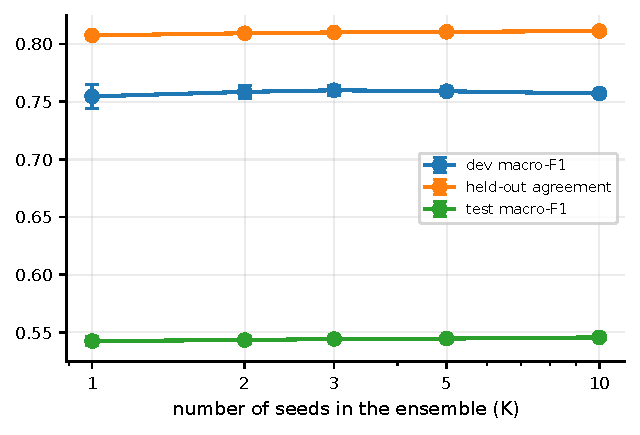
\includegraphics[width=0.85\columnwidth]{figures/fig_ensemble_size.pdf}
\caption{Effect of the table ensemble size (mean $\pm$ standard deviation over seed combinations).}
\label{fig:ensemble}
\end{figure}

\begin{figure}[!htbp]
\centering
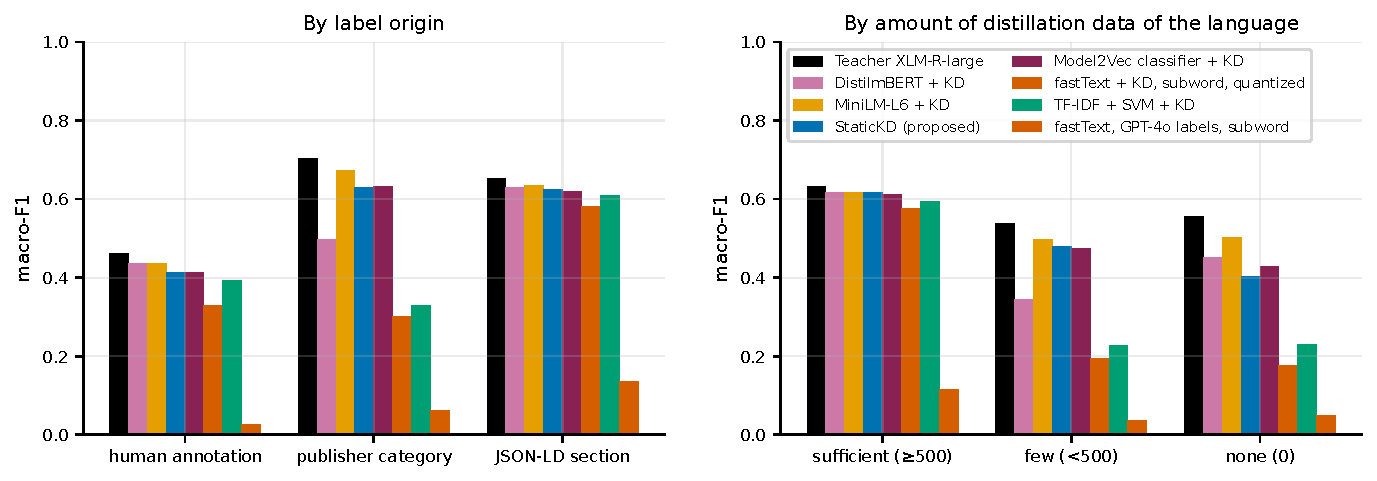
\includegraphics[width=0.78\textwidth]{figures/fig_groups.pdf}
\caption{Test macro-F1 by label origin (left) and by the amount of distillation data in the language of the article (right).}
\label{fig:groups}
\end{figure}

\begin{figure}[!htbp]
\centering
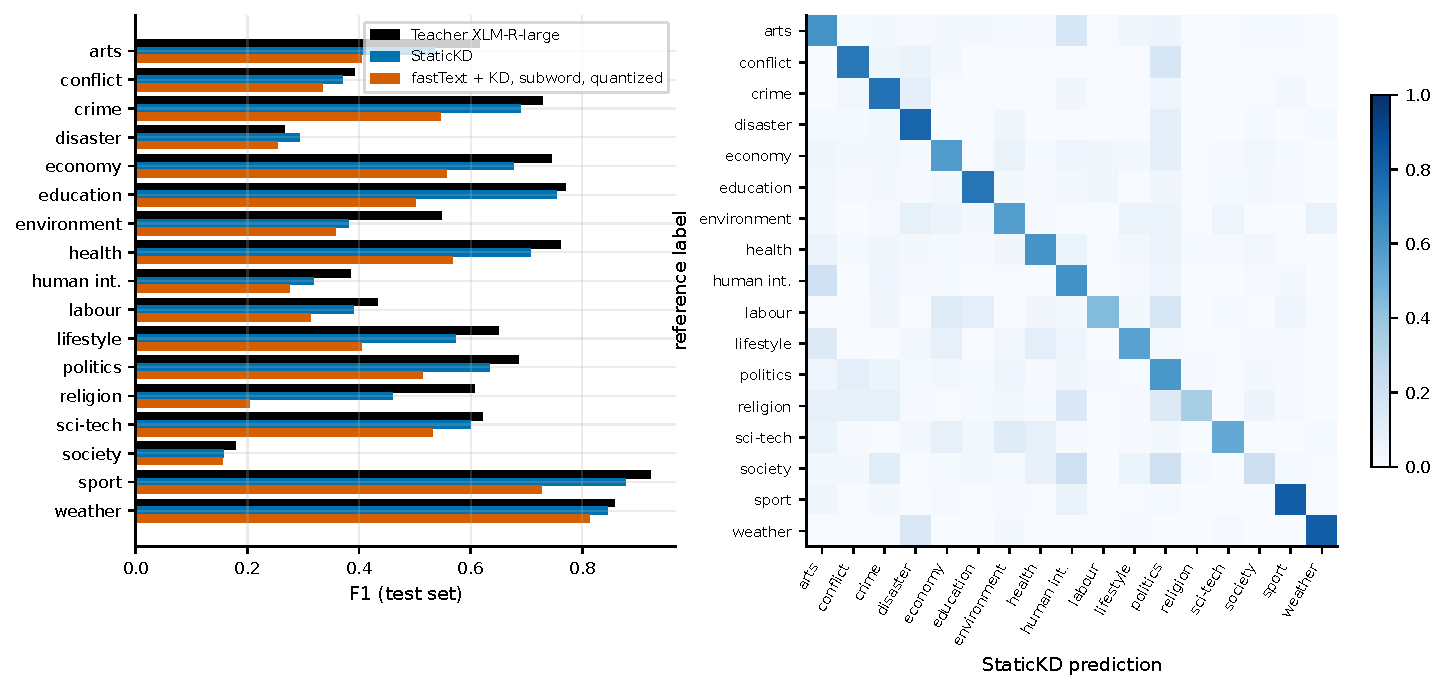
\includegraphics[width=0.9\textwidth]{figures/fig_per_label.pdf}
\caption{F1 per label on the test set (left) and the StaticKD confusion matrix normalized per reference label (right).}
\label{fig:label}
\end{figure}

\begin{figure}[!htbp]
\centering
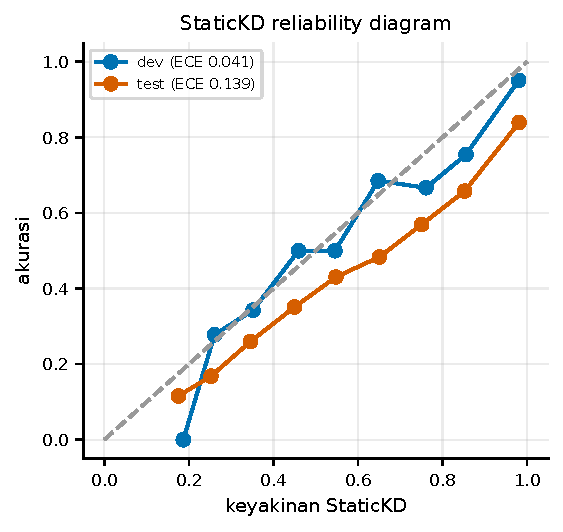
\includegraphics[width=0.8\columnwidth]{figures/fig_calibration.pdf}
\caption{Reliability diagram of StaticKD on the development and test sets.}
\label{fig:calib}
\end{figure}

\clearpage
\bibliographystyle{IEEEtran}
\bibliography{references}

\end{document}
